\subsection{Fluxions Isolation} \label{chapter5:flx:isolation}

As a rupture point occurs between an asynchronous caller and a callback defined \textit{in situ}, it eventually breaks the chain of scopes.
% A rupture point eventually breaks the chain of scopes between the upstream and downstream fluxion.
If the caller and the callback are separated, it breaks the closure of the callback.
The callback in the downstream fluxion cannot access the scope of its parent as expected. % in the upstream fluxion.
% The closure in the downstream fluxion cannot access the scope in the upstream fluxion as expected.
The pipeliner step replaces the need for this closure, allowing application parts to be isolated, and to rely only on independent memory stores and message passing.
It determines the distribution using the scope representation, which represents the variables' dependencies between application parts.
Depending on this representation, the compiler can replace the broken closures in three different ways.
We present these three alternatives in figure \ref{fig:states}.

\begin{figure}[h!]

\bigfig{
  \centering
  \parbox{\textwidth}{
    \parbox{0.40\textwidth}{
      \hfill
      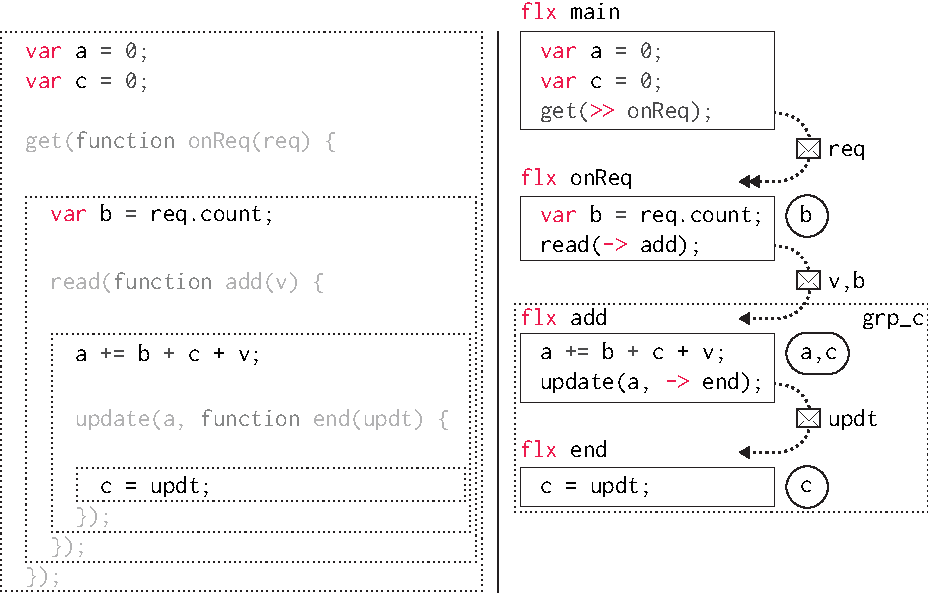
\includegraphics[page=1, height=0.4\textwidth]{../resources/states.pdf}
    }
    \hspace{10pt}
    $\to$
    \hspace{10pt}
    \parbox{0.40\textwidth}{
      \includegraphics[page=2, height=0.4\textwidth]{../resources/states.pdf}
      \hfill
    }
    \caption{Variable management from Javascript to the high-level fluxional language}
    \label{fig:states} 
  }
}

\end{figure}

\subsubsection{Scope}
If a variable is modified inside only one application part in the current \textit{post} chain, then the pipeliner adds it to the context of its fluxion.

In figure \ref{fig:states}, the variable \texttt{a} is updated in the function \texttt{add}.
The pipeliner step stores this variable in the context of the fluxion \texttt{add}.

\subsubsection{Stream}
If a modified variable is read by some downstream application parts, then the pipeliner makes the upstream fluxion add this variable to the message stream to be sent to the downstream fluxions.
It is impossible to send variables to upstream flux\-ions, without causing inconsistencies.
If the fluxion retro propagates the variable for an upstream fluxion to read, the upstream fluxion might use the old version while the new version is on its way.

In figure \ref{fig:states}, the variable \texttt{b} is set in the function \texttt{onReq}, and read in the function \texttt{add}.
The pipeliner step makes the fluxion \texttt{onReq} send the updated variable \texttt{b}, in addition to the variable \texttt{v}, in the message sent to the fluxion \texttt{add}.

Exceptionally, if a variable is defined inside a \textit{post} chain, like \texttt{b}, then this variable can be streamed inside this \textit{post} chain without restriction on the order of modification and read.
Indeed, in the current \textit{post} chain, the execution of the upstream fluxion is assured to end before the execution of the downstream fluxion, because of their causality.
Therefore, no reading of the variable by the upstream fluxion happens after the modification by the downstream fluxion.

\subsubsection{Share}
If a variable is needed for modification by several application parts, or is read by an upstream application part, then it needs to be synchronized between the fluxions.
% To respect the semantics of the source application, we cannot tolerate inconsistencies.
The pipeliner groups all the fluxions sharing this variable with the same tag.
And it adds this variable to the contexts of each fluxions.

In figure \ref{fig:states}, the variable \texttt{c} is set in the function \texttt{end}, and read in the function \texttt{add}.
As the fluxion \texttt{add} is upstream of \texttt{end}, the pipeliner step groups the fluxion \texttt{add} and \texttt{end} with the tag \texttt{grp\_c} to allow the two fluxions to share this variable.